\documentclass[a4paper,12pt]{article}
\usepackage[section]{placeins}
\usepackage{tikz}		
\usepackage{url}
\usepackage{amsmath}
\usepackage{graphicx}
\usepackage{pgfplots}
\usepackage{listings}
\usepackage{hyperref}
\usepackage[czech]{babel}

\author{Moravec Vojtěch}
\title{Analýza sítě odpovědí na stránce \emph{MathOverflow}}
\date{Zimní semestr 2018}

\begin{document}

\maketitle
\newpage

\section{Popis datasetu}

Analyzovaný dataset byl získán ze stránky \emph{snap.stanford.edu} \cite{snapnets}. Dataset obsahuje
seznam hran orientovaného neohodnoceného grafu, který reprezentuje interakci mezi uživateli stránky
 \emph{https://mathoverflow.net/}. Hrana ($u$,$v$) vycházející z vrcholu $u$ do vrcholu $v$, znamená, že
 uživatel $u$ odpověděl na otázku uživatele $v$. Originální dataset obsahuje také časové razítka vzniku
 hrany, ale pro naše účely je budeme ignorovat a budeme pracovat se všemi hranami.
 
\section{Analýza sítě}
Síť obsahuje $21 688$ vrcholů a $107 581$ hran, tedy $21 668$ uživatelů a $107 581$ odpovědí na otázky.

\subsubsection{Analýza stupňů vrcholů}
\begin{table}[h!]
\centering
\begin{tabular}{l | r | r | r | r | r}
 				& Minimum & Výskyt	& Maximum & Výskyt	& Průměr \\
\hline
Vstupní stupeň 	& 0 & $5683 \times$	& 1102 	& 	$1 \times$	& 4,9604 \\
Výstupní stupeň & 0 & $11309 \times$& 1415 	& 	$1 \times$	& 4,9603 \\
Celkový stupeň  & 1	& $9445 \times$	& 1815	&	$1 \times$	& 9,9207
\end{tabular}
\caption{Tabulka stupňů vrcholů}
\label{tab:degree}
\end{table}

Z Tabulky \ref{tab:degree} můžeme vyčíst, tyto extrémy:
\begin{itemize}
\item 5683 uživatelům nepřišla žádná odpověď na jejich otázky.
\item Jednomu uživateli přišlo celkem 1102 odpovědí na jeho otázky.
\item 11309 uživatelů neposkytlo žádnou odpověď.
\item Nejvíce odpovědí napsal jeden uživatel a to 1415 odpovědí.
\end{itemize}

Průměrný uživatel napsal skoro 5 odpovědí na otázky ostatních a taktéž průměrně získal 5 odpovědí 
od ostatních uživatelů. Větší výstupní stupeň v této sítí naznačuje, že daný uživatel je vlivným 
vzhledem k této komunitě.

Dále na Obrázcích \ref{img:all_deg_rel}, \ref{img:out_deg_rel} a \ref{img:in_deg_rel} můžeme 
v grafech vidět relativní distribuci stupňů. Tato distribuce odpovídá mocninnému dělení, 
jak je tomu u obecně reálných sítí. Na Obrázcích \ref{img:all_deg_cum}, \ref{img:out_deg_cum} a
\ref{img:in_deg_cum} můžeme vidět kumulativní distribuci stupňů.

% RELATIVNI DISTRIBUCE
\begin{figure}[h!]
\centering
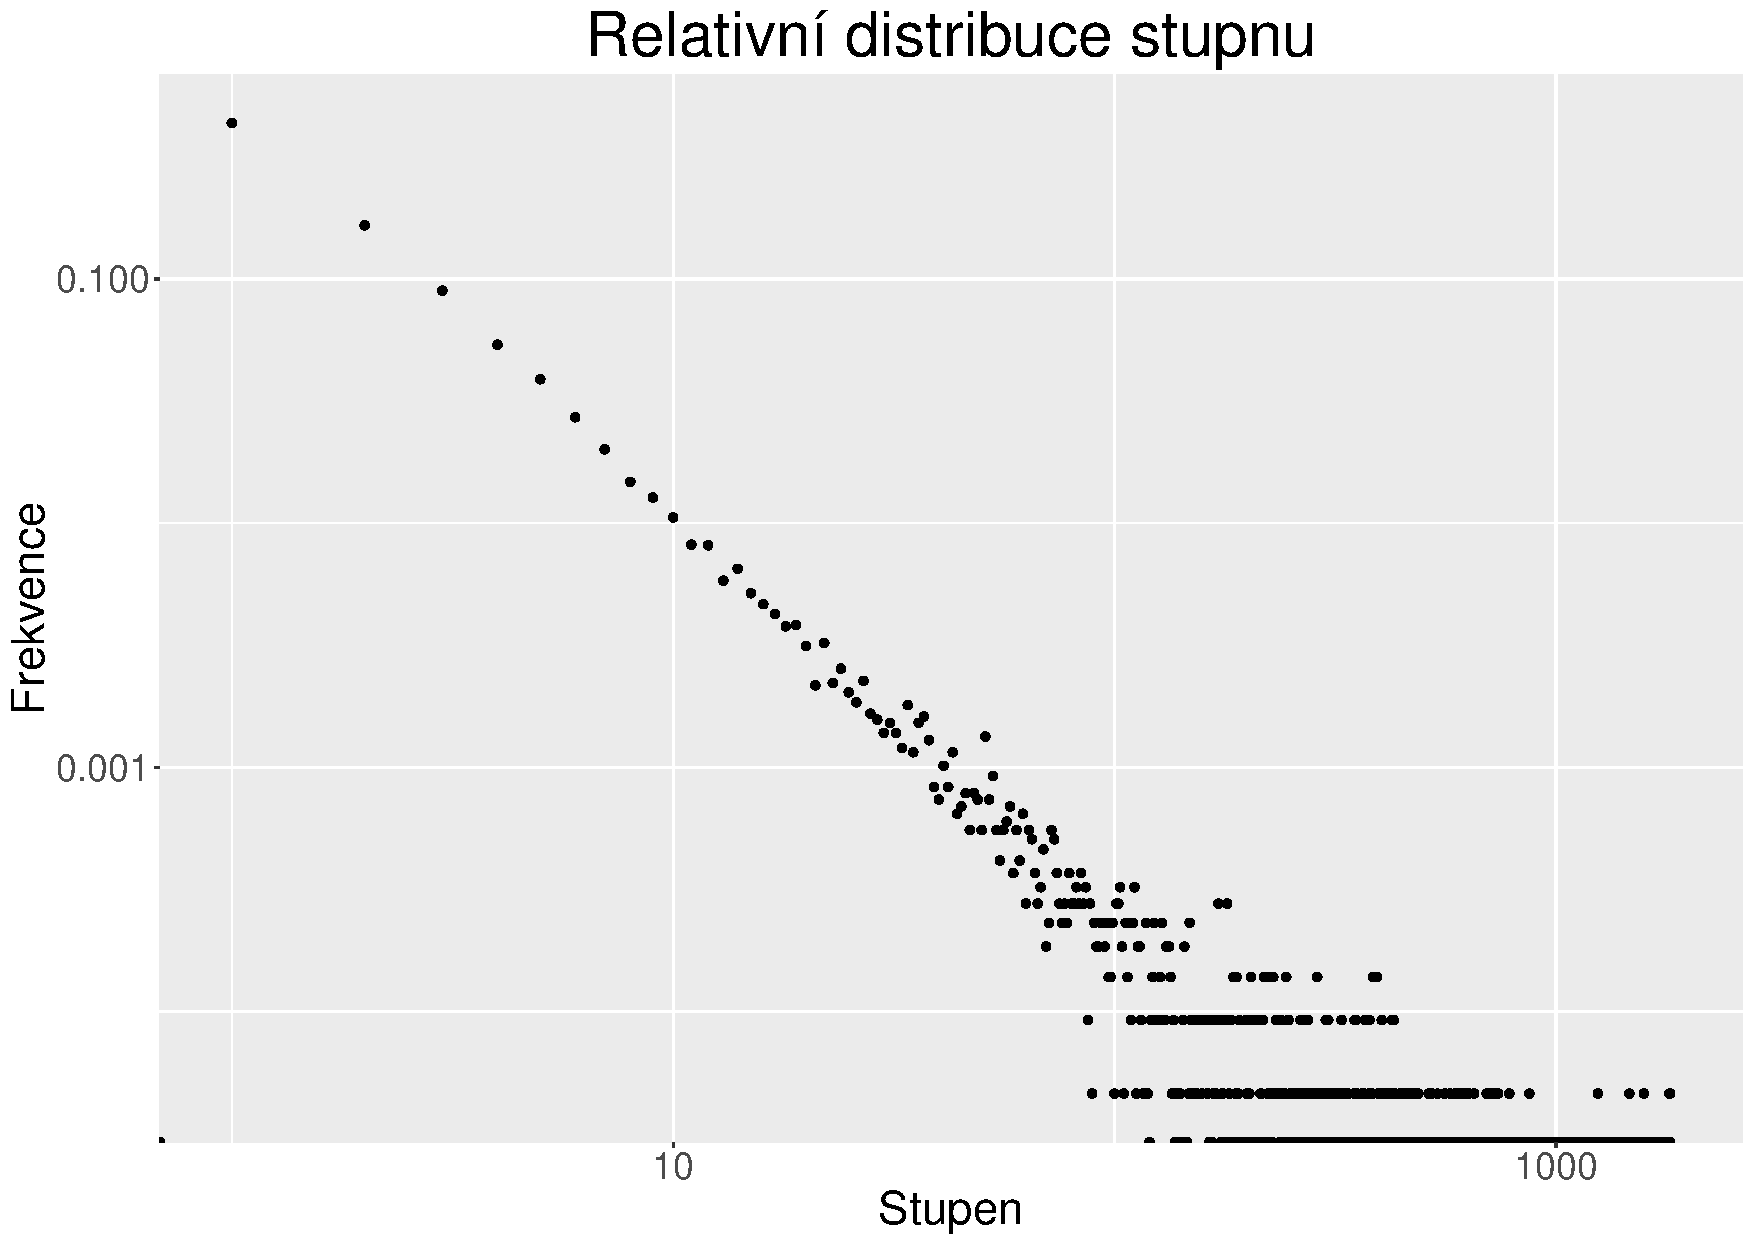
\includegraphics[scale=0.4]{images/all_deg_rel.pdf}
\caption{Graf relativní distribuce stupňů}
\label{img:all_deg_rel}
\end{figure}

\begin{figure}[h!]
\centering
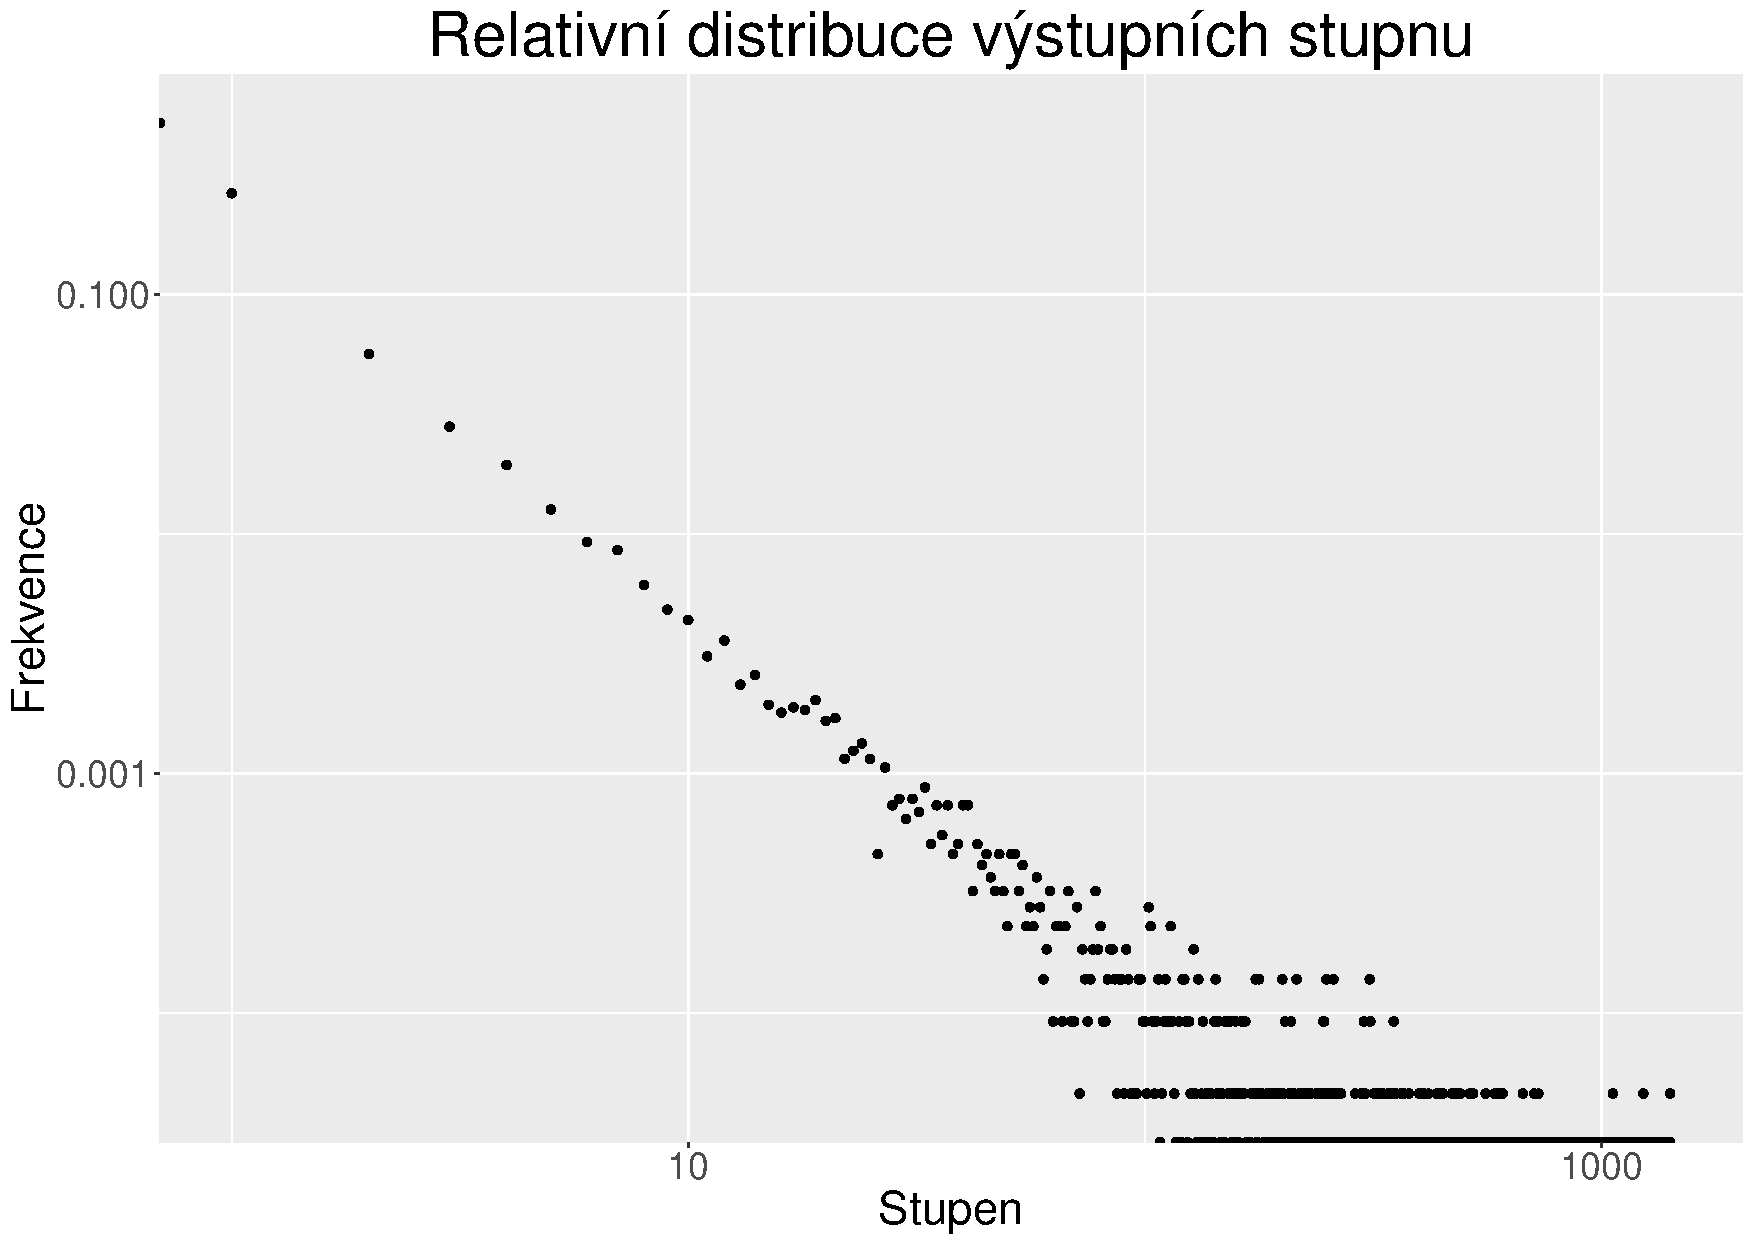
\includegraphics[scale=0.4]{images/out_deg_rel.pdf}
\caption{Graf relativní distribuce výstupních stupňů}
\label{img:out_deg_rel}
\end{figure}


\begin{figure}[h!]
\centering
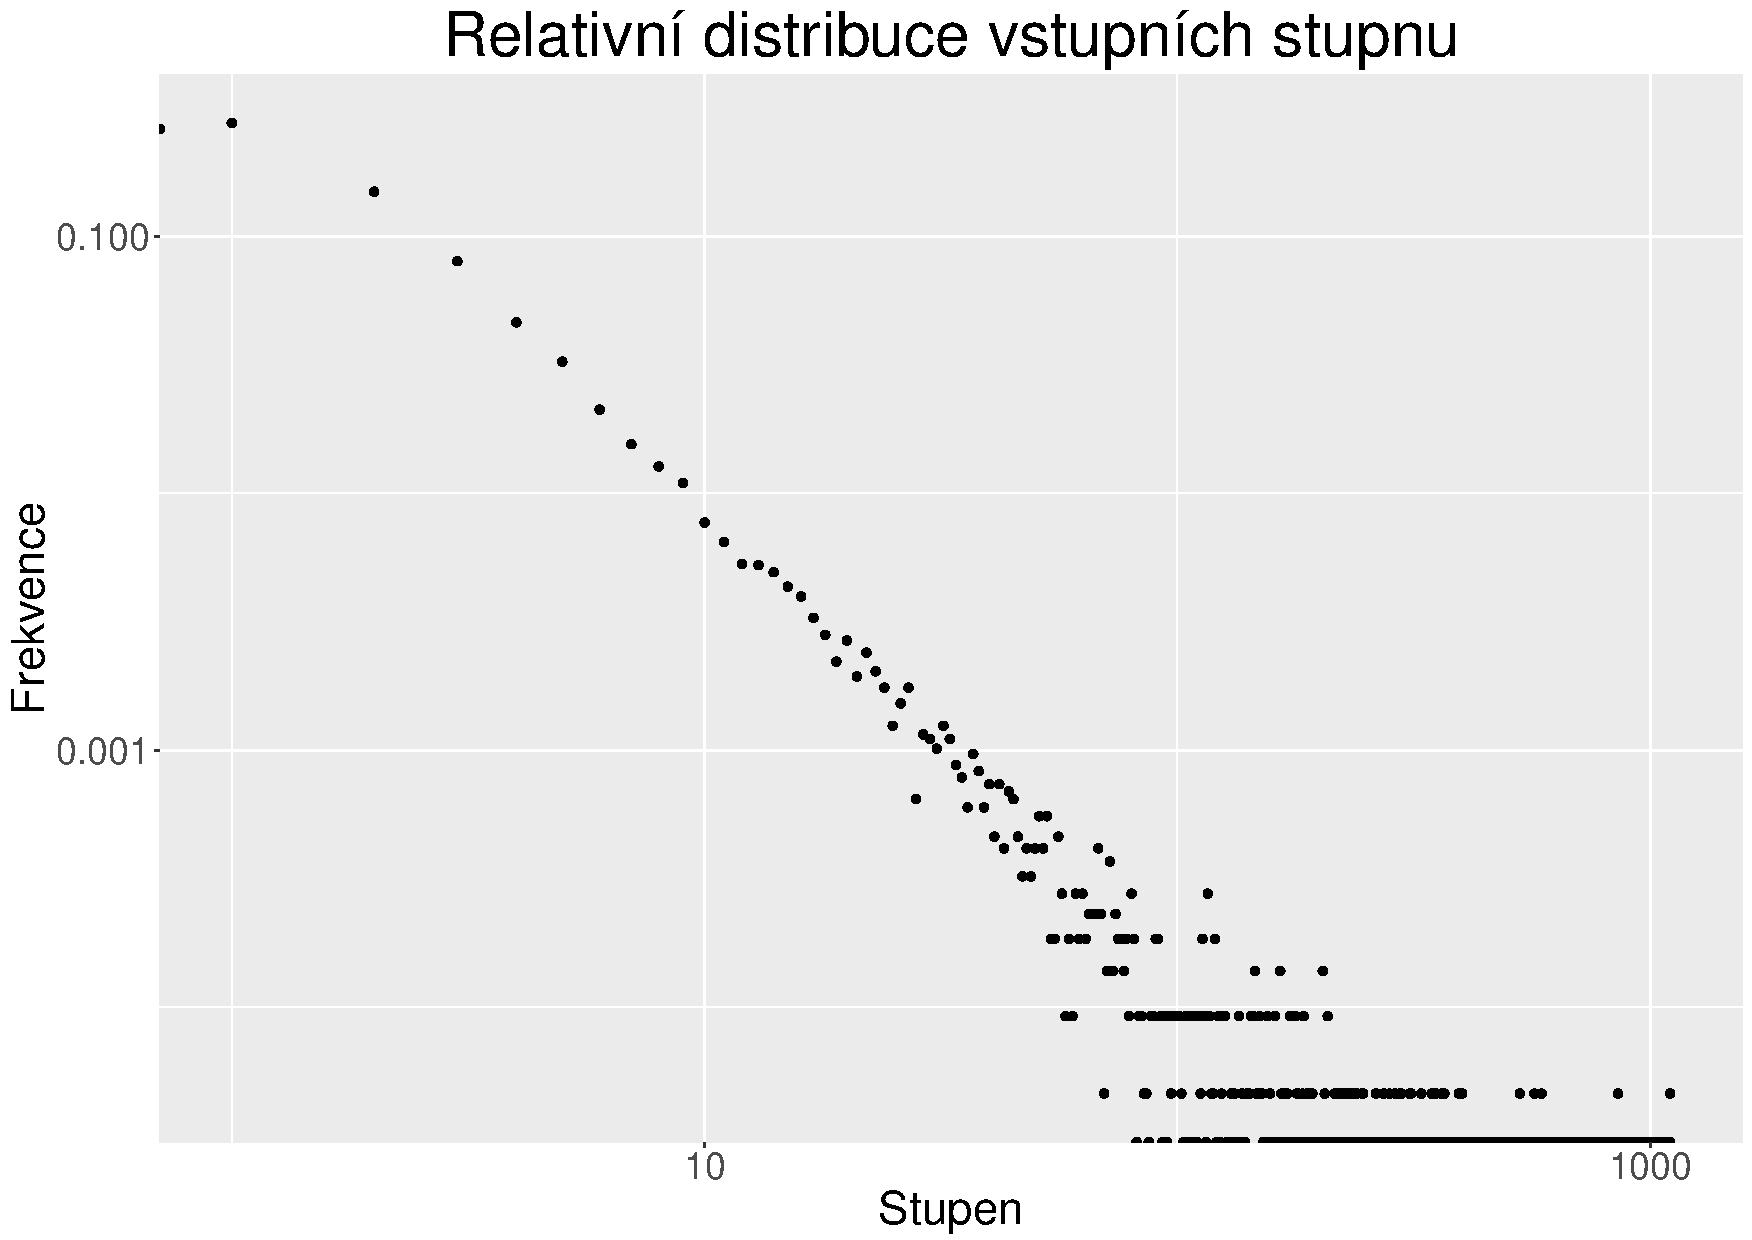
\includegraphics[scale=0.4]{images/in_deg_rel.pdf}
\caption{Graf relativní distribuce vstupních stupňů}
\label{img:in_deg_rel}
\end{figure}

% KUMULATIVNI DISTRIBUCE
\begin{figure}[h!]
\centering
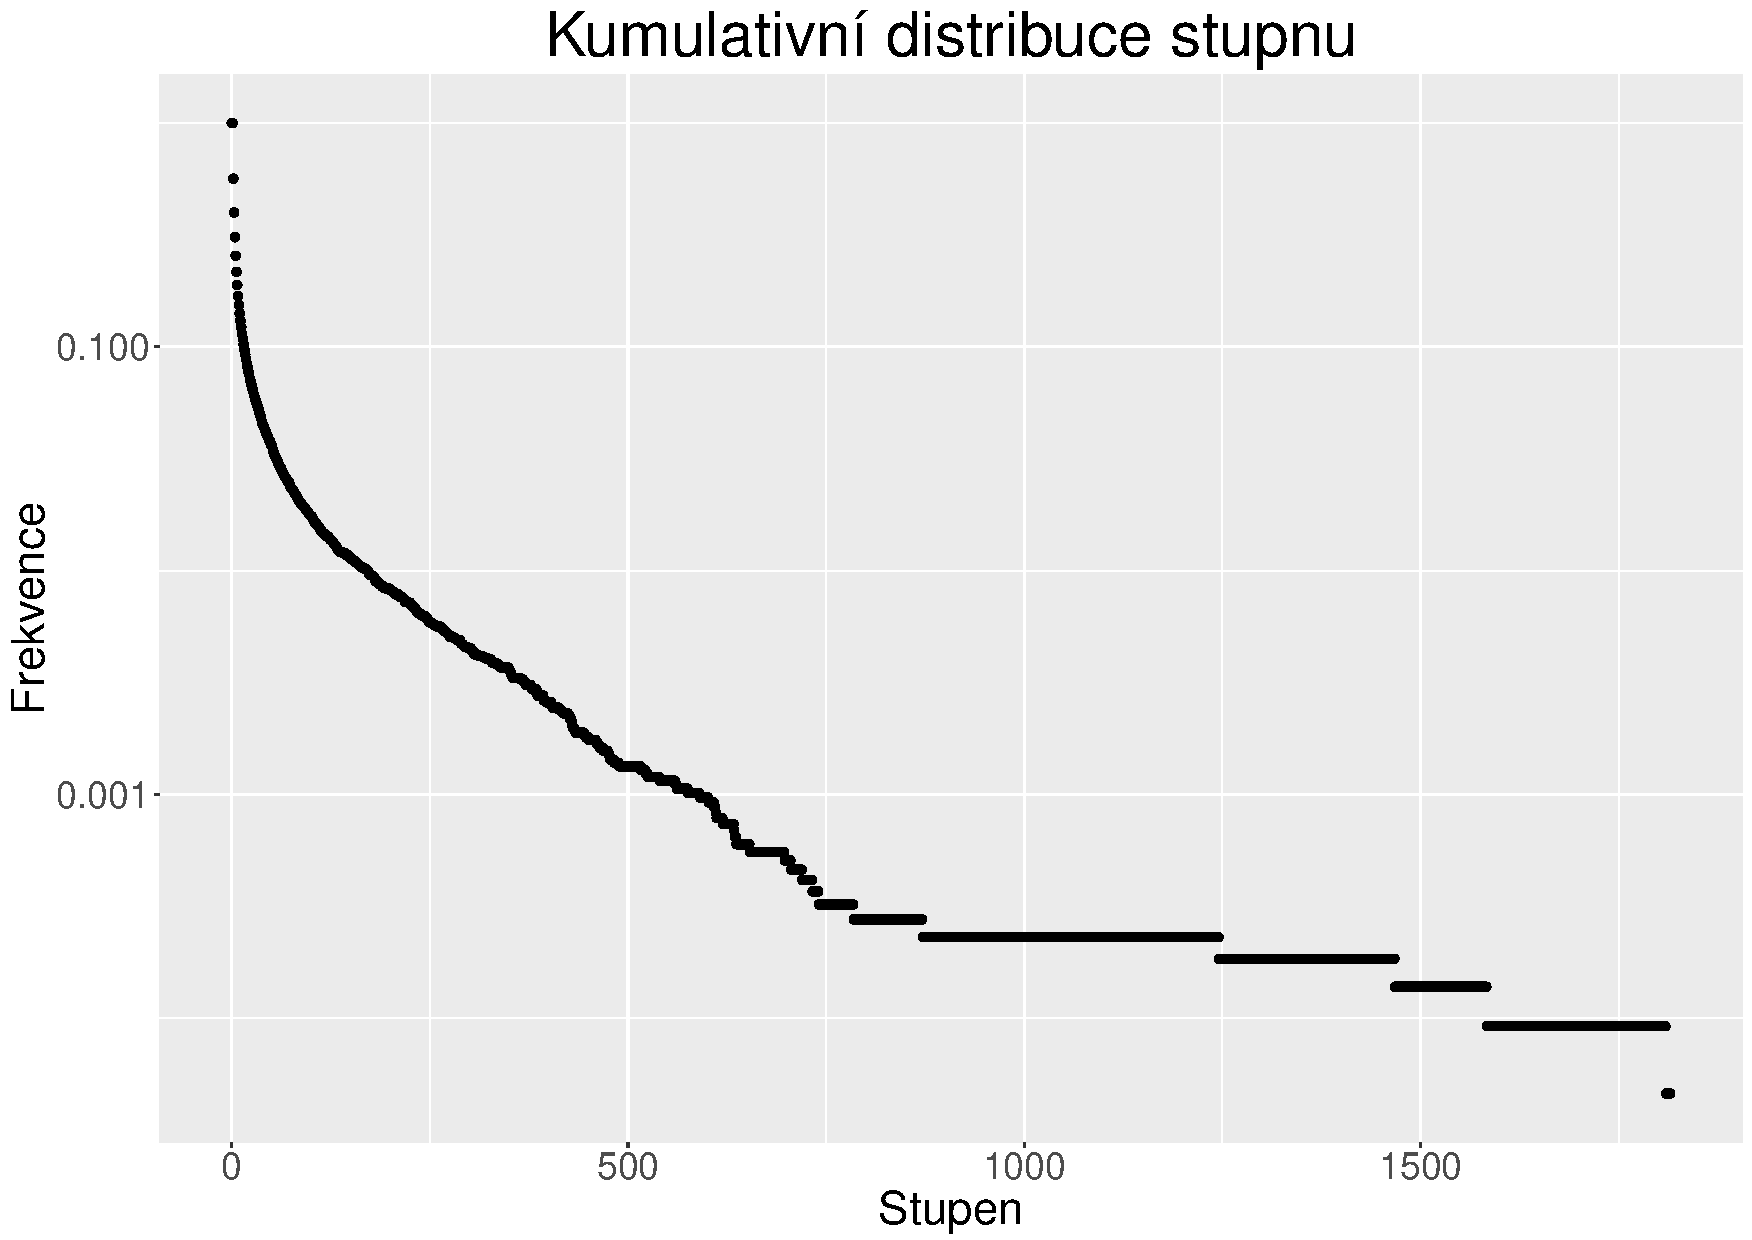
\includegraphics[scale=0.4]{images/all_deg_cum.pdf}
\caption{Graf kumulativní distribuce stupňů}
\label{img:all_deg_cum}
\end{figure}



\begin{figure}[h!]
\centering
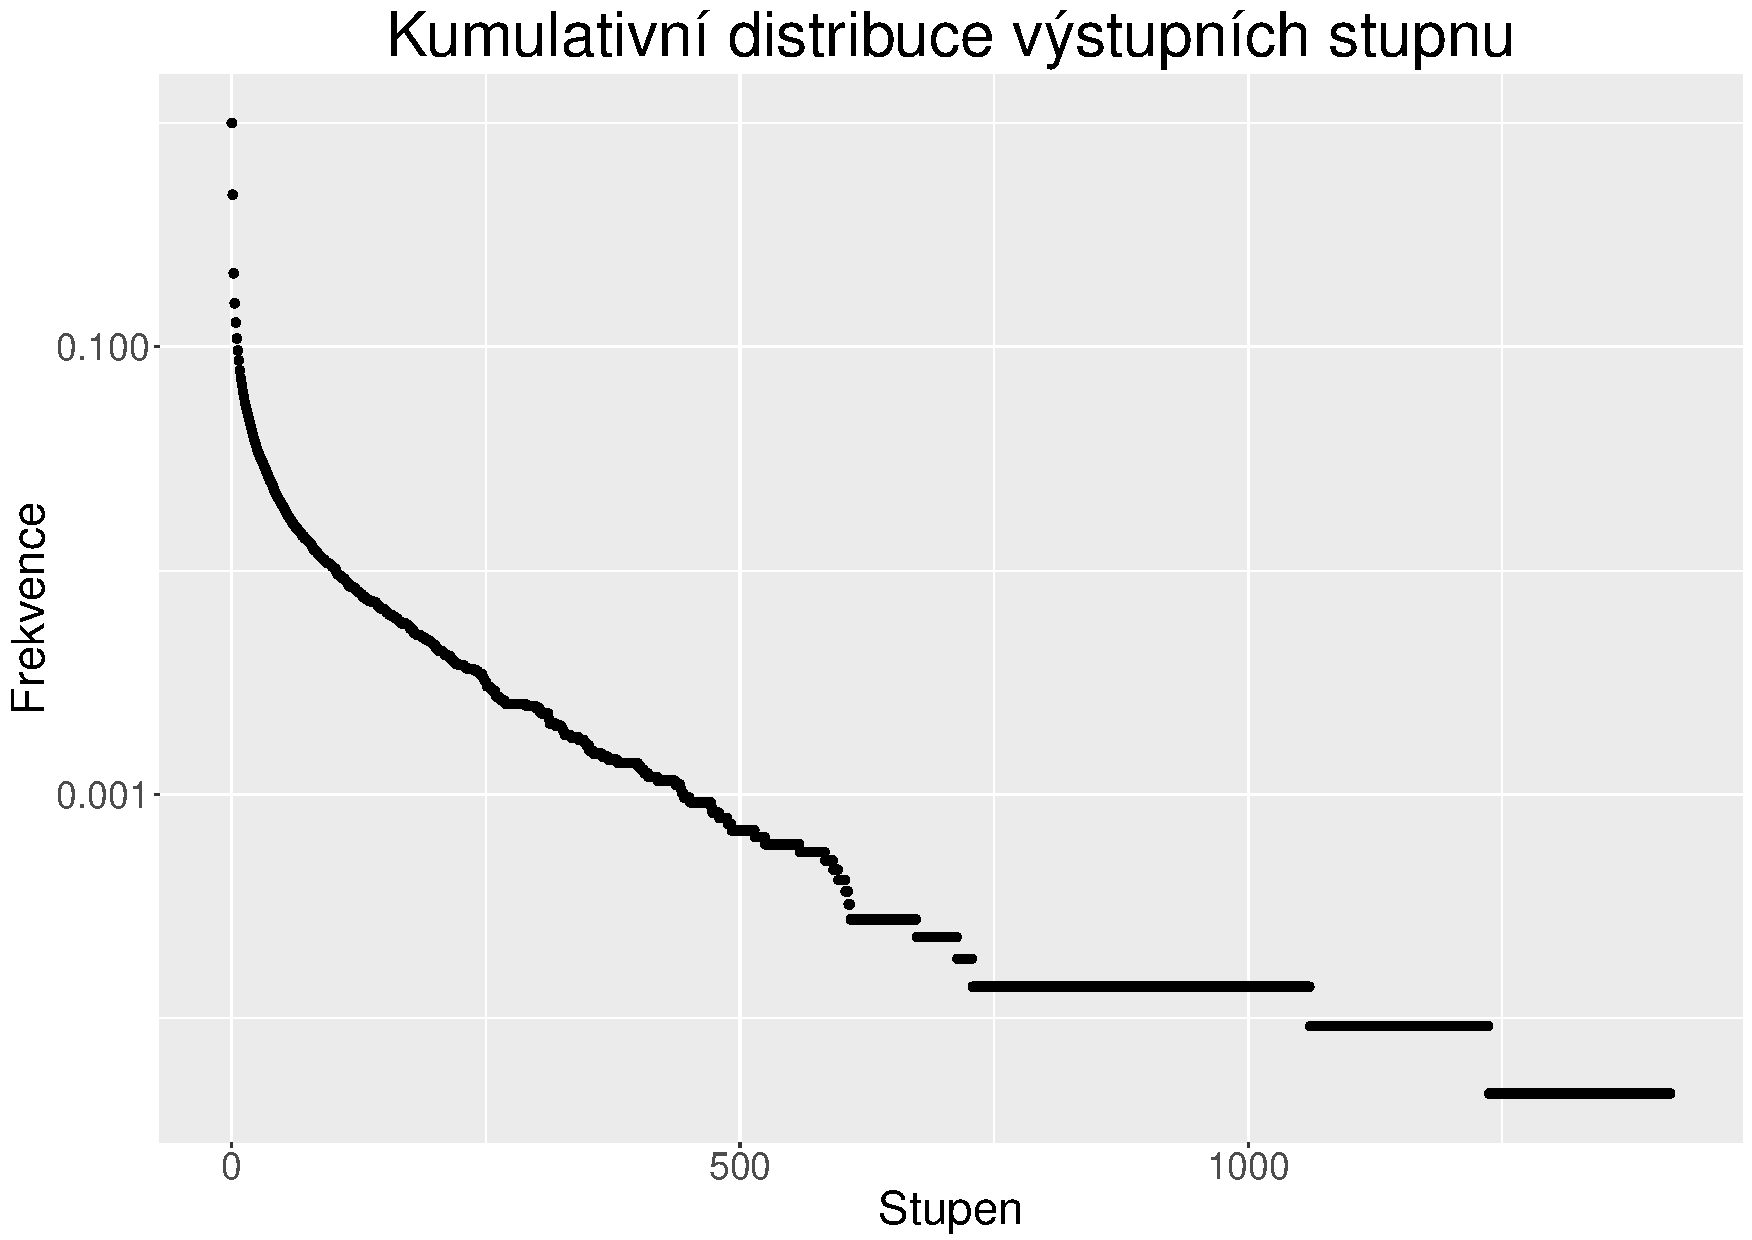
\includegraphics[scale=0.4]{images/out_deg_cum.pdf}
\caption{Graf kumulativní distribuce výstupních stupňů}
\label{img:out_deg_cum}
\end{figure}

\begin{figure}[h!!]
\centering
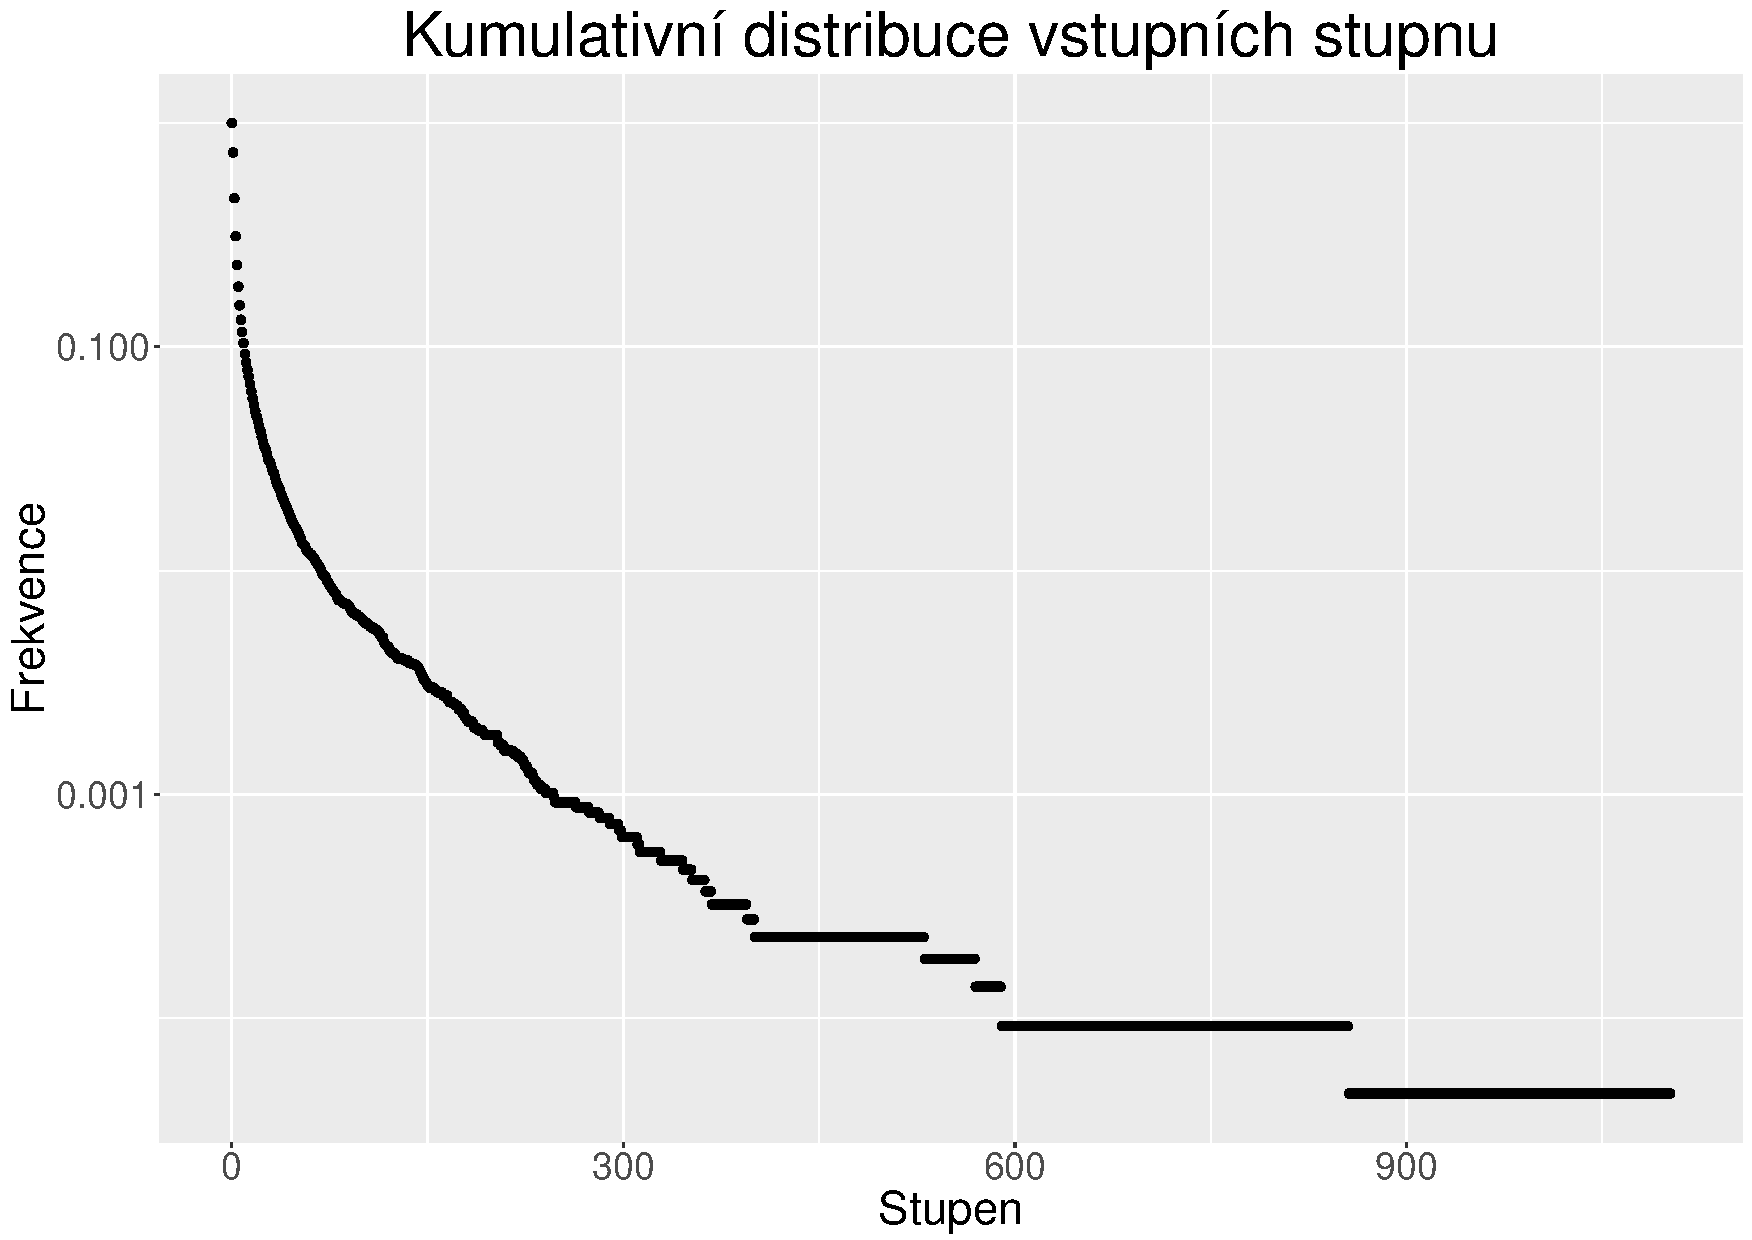
\includegraphics[scale=0.4]{images/in_deg_cum.pdf}
\caption{Graf kumulativní distribuce vstupních stupňů}
\label{img:in_deg_cum}
\end{figure}

\FloatBarrier


\newpage
\subsubsection{Analýza cest v síti}
Průměr sítě neboli, nejdelší z nejkratších cest mezi vrcholy, je v naší sítí roven 17. 
Cesta v našem grafu značí posloupnost uživatelů, kteří si odpověděli na otázku. Průměrná délka nejkratší cesty je 4,18. Uživatelé jsou tedy průměrně spojeni přes 4,18 dalších uživatelů.

V grafu na Obrázku \ref{img:eccen} můžeme vidět výstupní excentricitu jednotlivých vrcholů. Excentricita je 
vzdálenost nejkratší cesty k nejvzdálenějšímu vrcholu. $11947$ vrcholů z celkového počtu $21688$ 
vrcholů má nulovou excentricitu, což znamená, že jsou izolované, neexistuje z nich cesta do ostatních
vrcholů. Jsou to tzv. pasivní uživatelé.


\begin{figure}[h!]
\centering
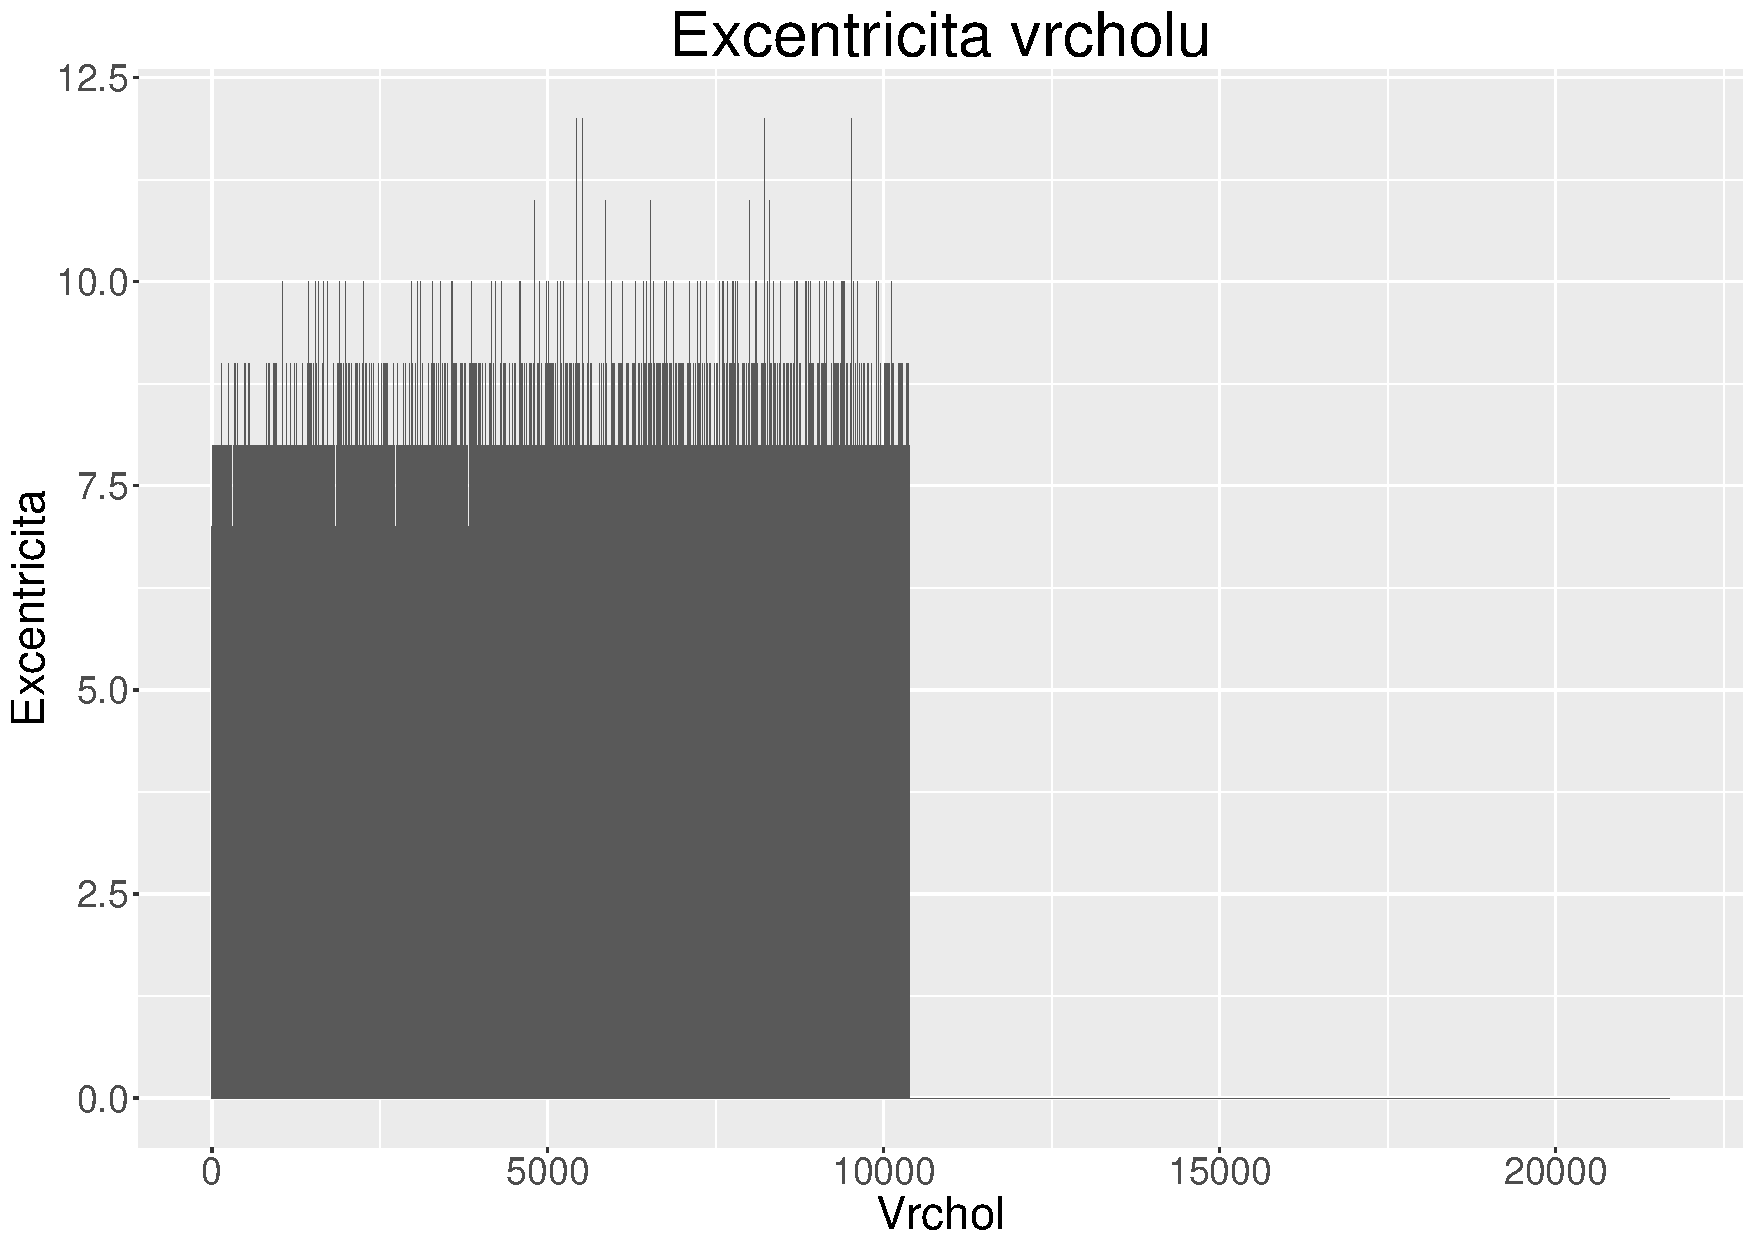
\includegraphics[scale=0.4]{images/eccen.pdf}
\caption{Excentricita vrcholů grafu}
\label{img:eccen}
\end{figure}

\FloatBarrier
\subsubsection{Centrality v síti}

Jak už jsme pozorovali u excentricity, uživatelé se dělí na aktivní a pasivní. V grafu na Obrázku
\ref{img:close} můžeme vidět closeness centralitu. Vrcholy jsou zde rozděleny do dvou různých skupin.
Na Obrázcích \ref{img:bc} a \ref{img:bc_log} vidímě betweenness centrality. Více toho vyčteme na grafu
s logaritmickou osou $y$. Betweenness a Closeness centralita mezi sebou korelují, neboť obě pozorují 
2 velmi rozdílné skupiny vrcholů.

\begin{figure}[h!]
\centering
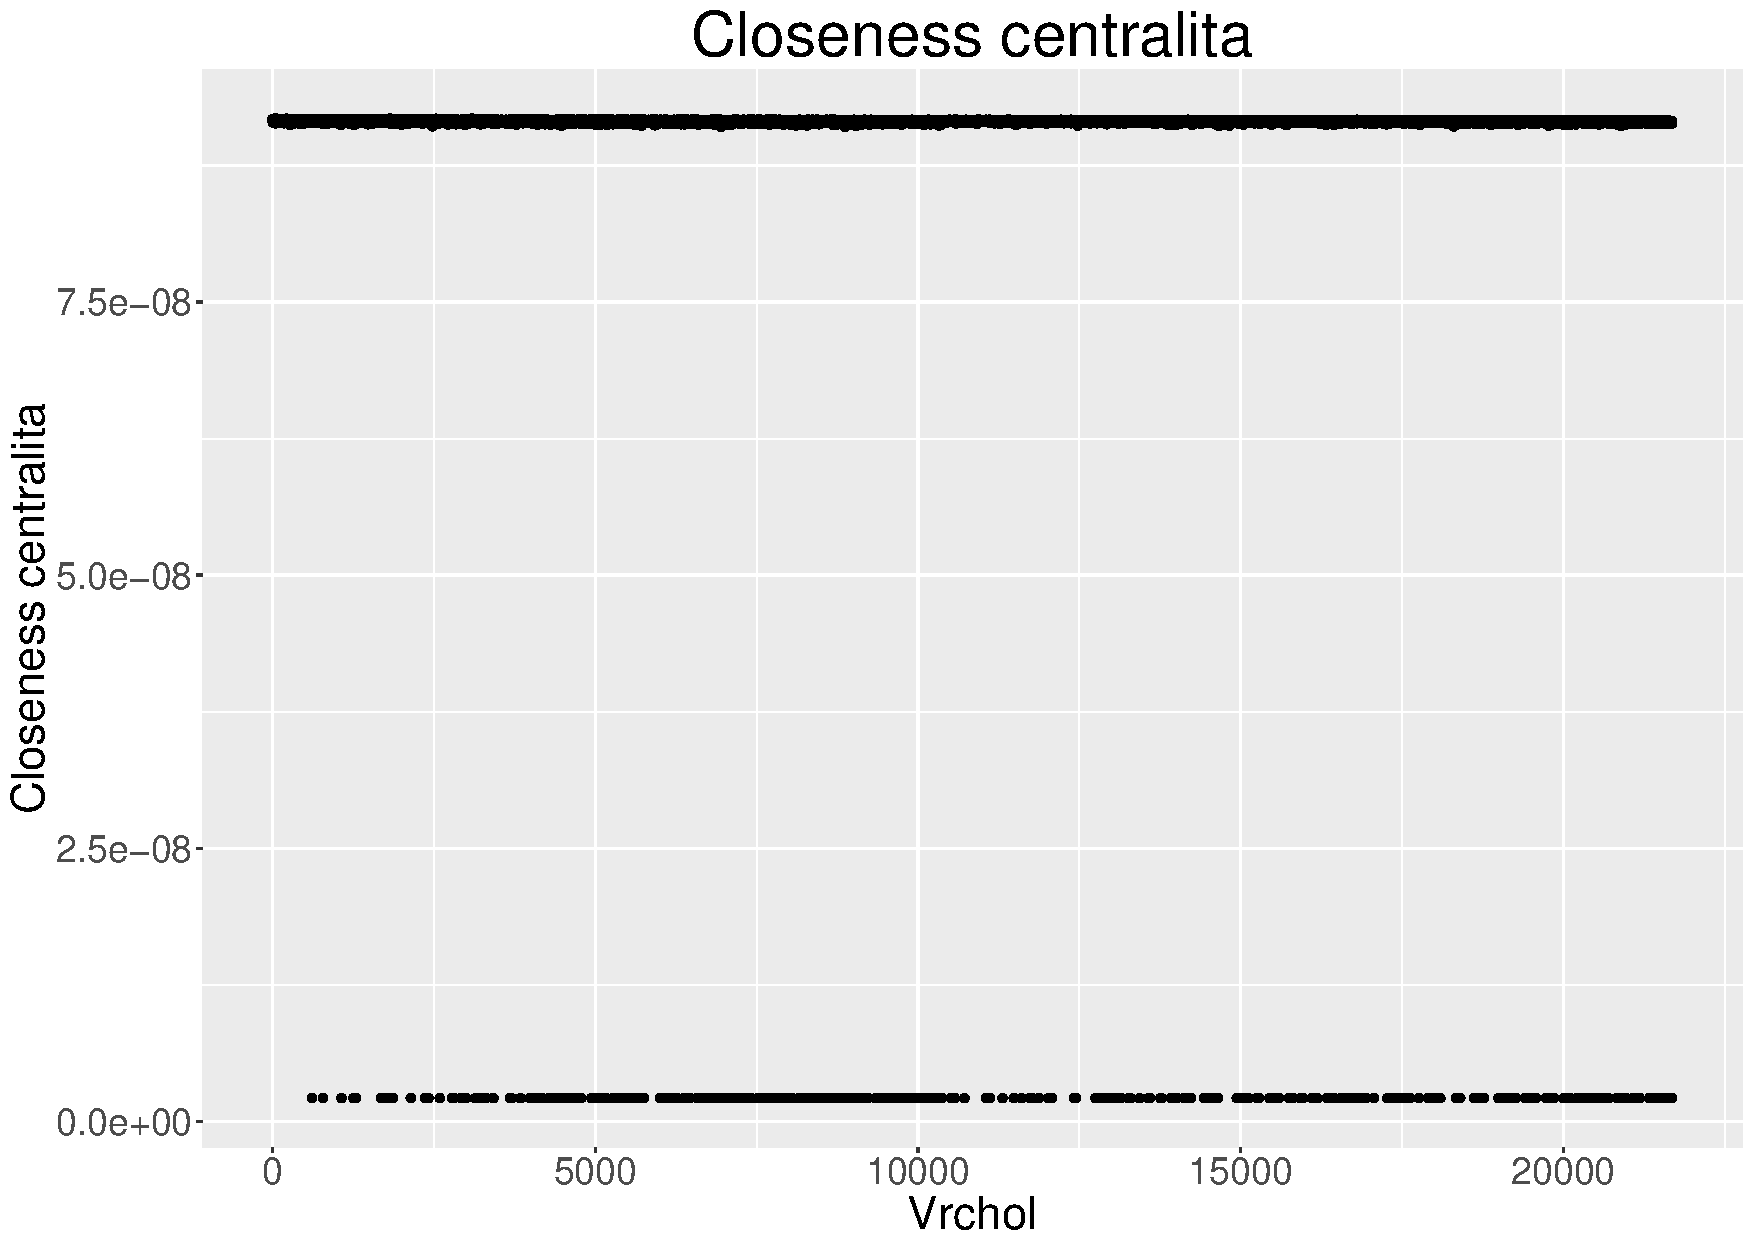
\includegraphics[scale=0.4]{images/closeness.pdf}
\caption{Closeness centralita}
\label{img:close}
\end{figure}

\begin{figure}[h!]
\centering
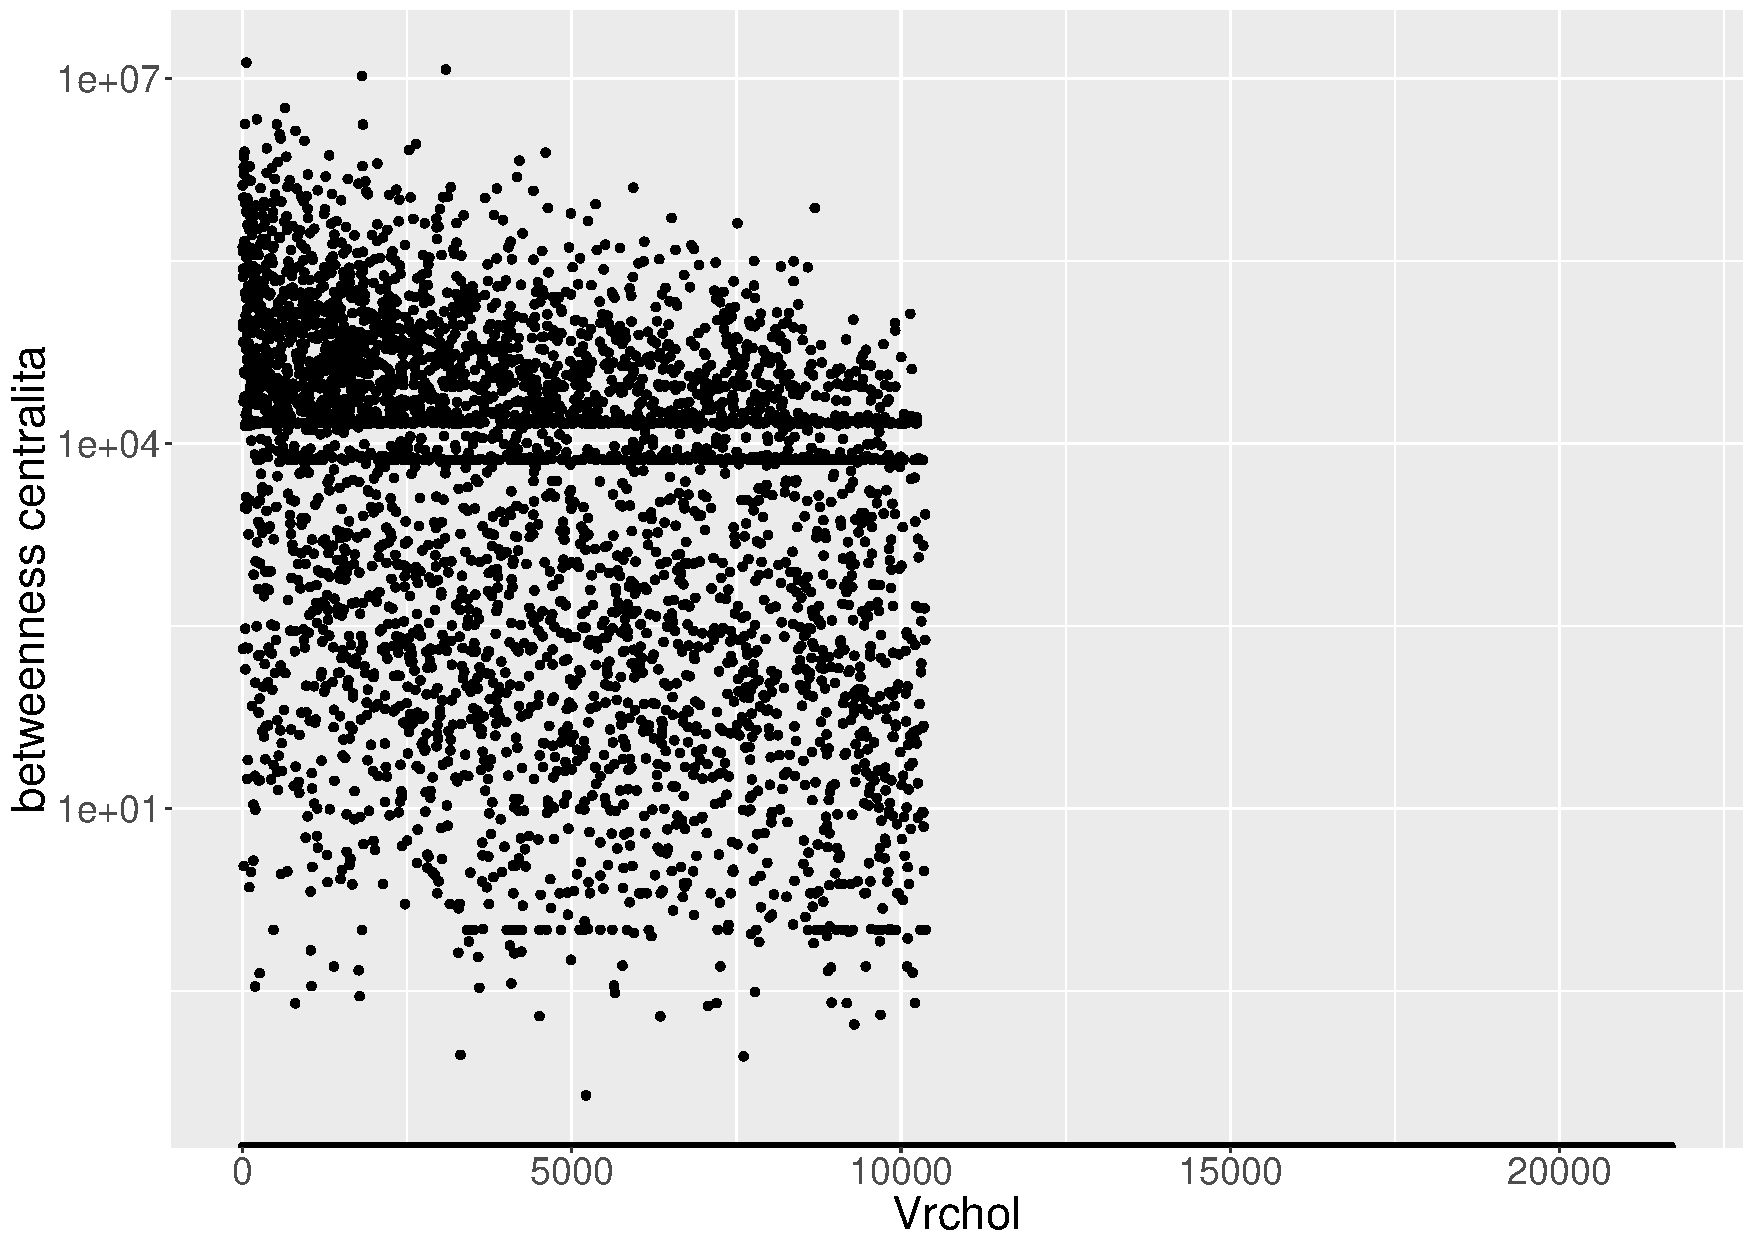
\includegraphics[scale=0.4]{images/betweenness.pdf}
\caption{Betweenness centralita}
\label{img:bc}
\end{figure}

\begin{figure}[h!]
\centering
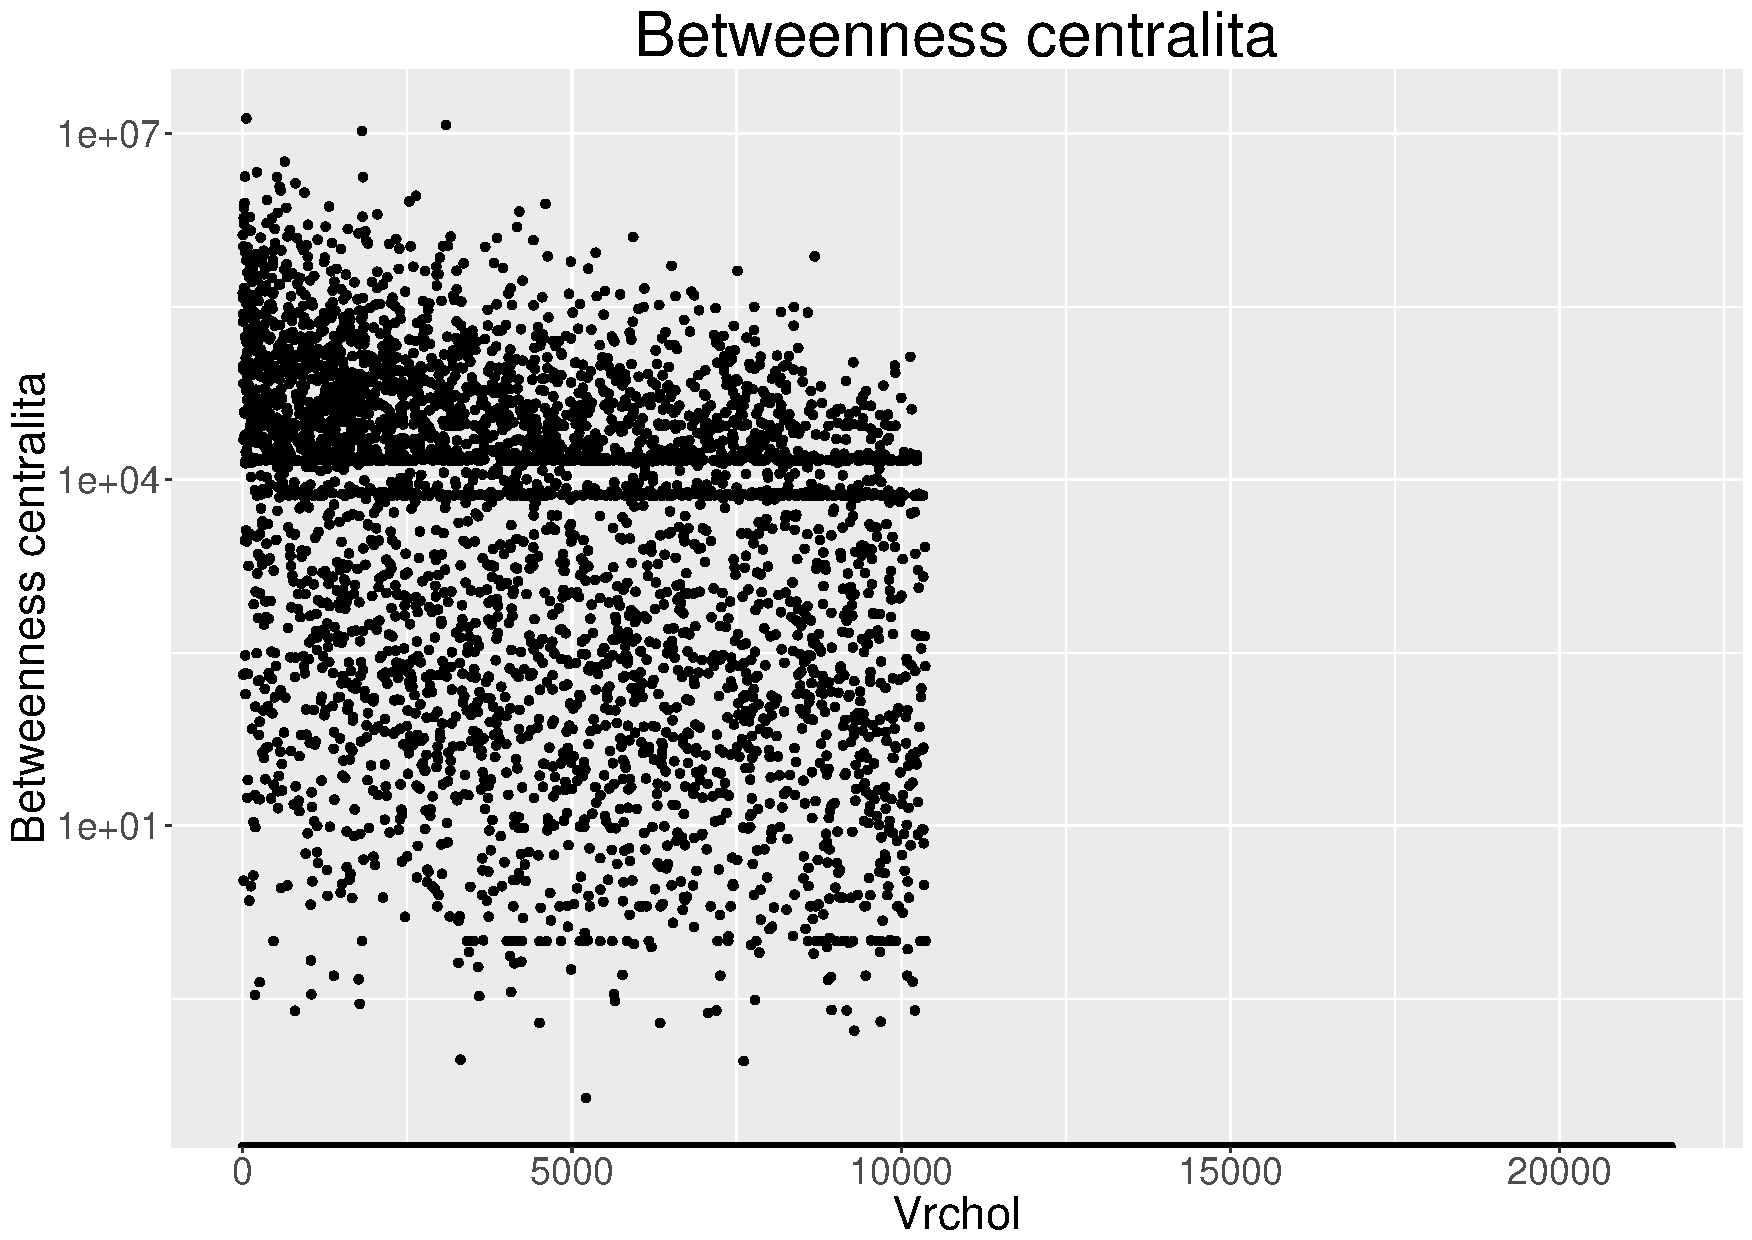
\includegraphics[scale=0.4]{images/betweenness_log.pdf}
\caption{Betweenness centralita v logaritmickém měřítku}
\label{img:bc_log}
\end{figure}

Jako další dvě centrality zde máme Kleinbergovu hub centralitu \ref{img:hubs}, která přiřazuje
vyšší hodnoty těm vrcholům, s více výstupními hranami, tedy těm uživatelům, kteří více odpovídají
na otázky. Zase zde vidíme rozdělení na aktivnější uživatele v odpovídání a ty pasivnější. 
Druhou centralitou je Kleinbergova autority centralita \ref{img:autority}, ta přiřazuje vyšší hodnoty
naopak těm s vrcholům s více vstupním hranami.

\begin{figure}[h!]
\centering
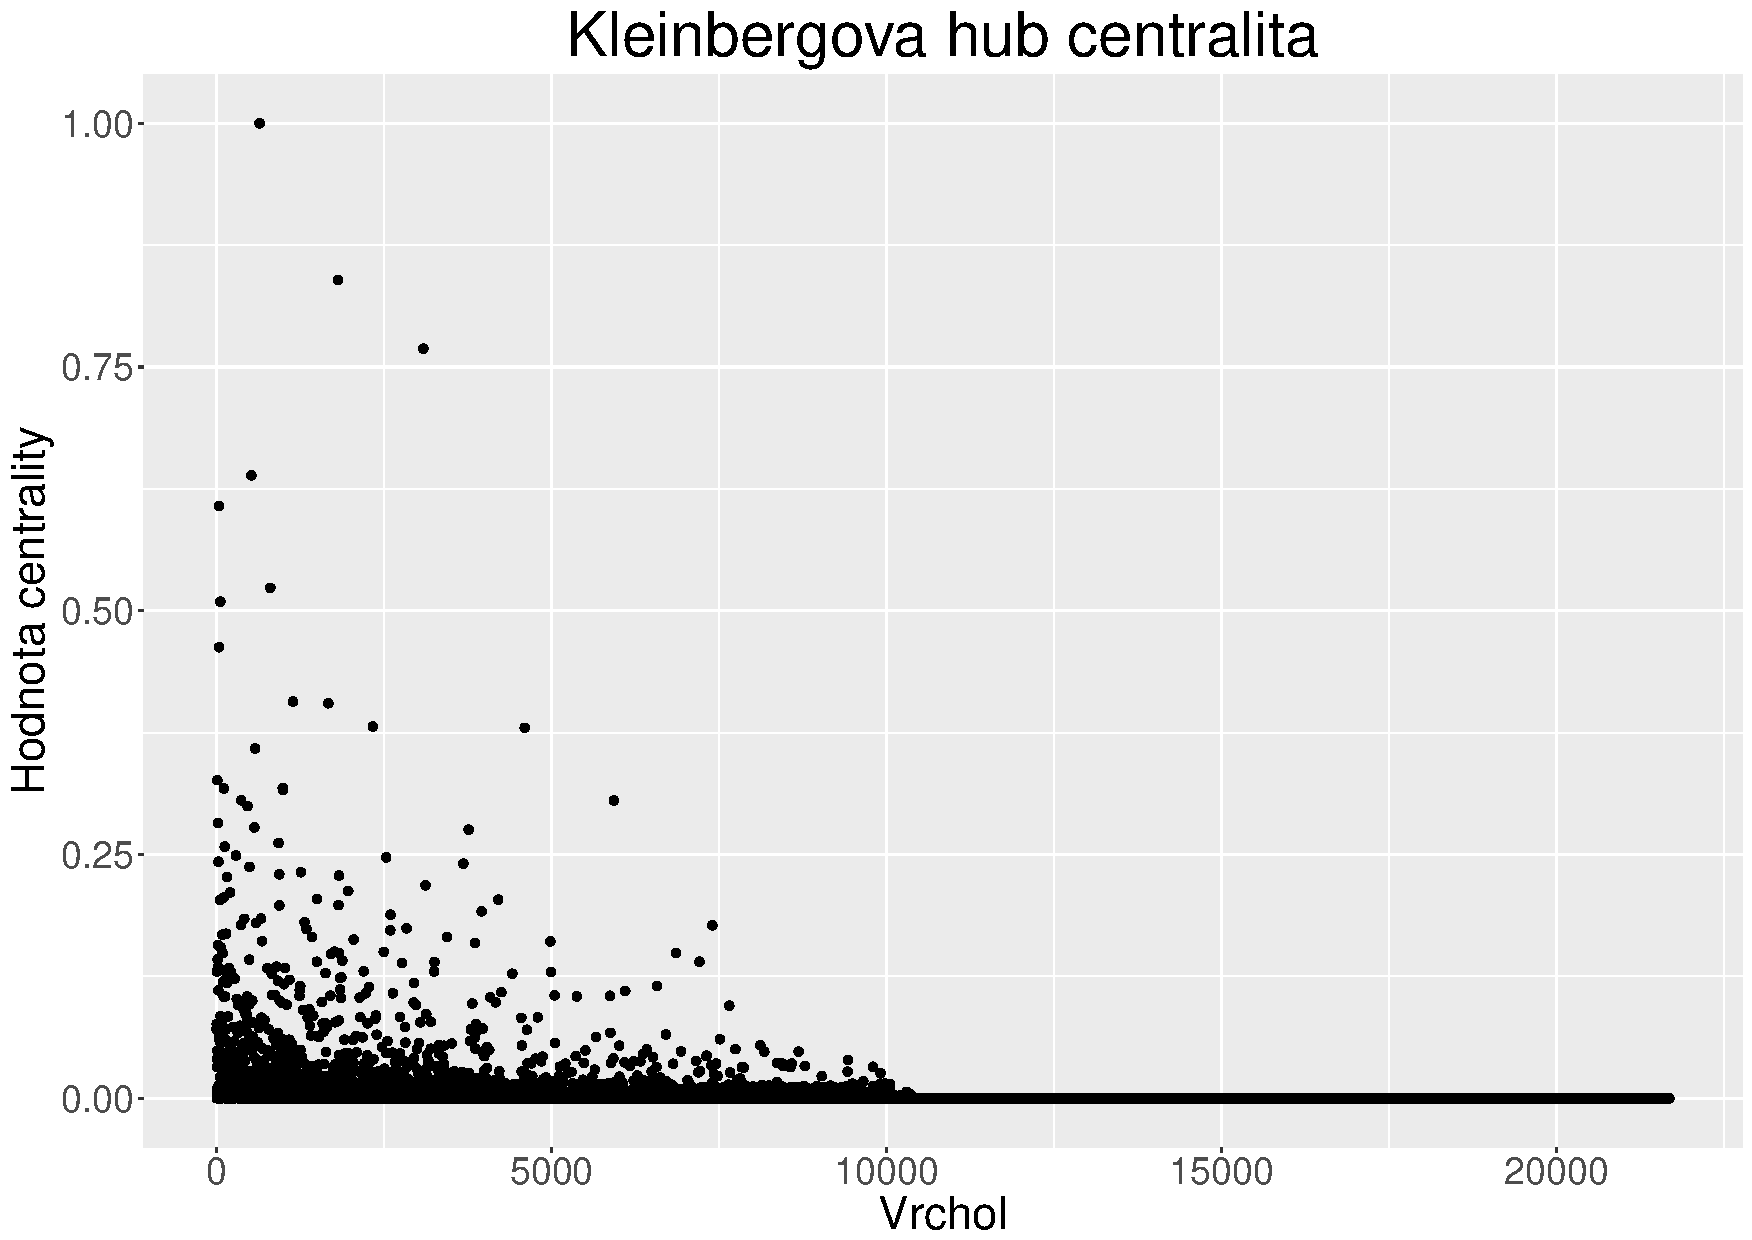
\includegraphics[scale=0.4]{images/hubs.pdf}
\caption{Kleinbergova hubs centralita}
\label{img:hubs}
\end{figure}

\begin{figure}[h!]
\centering
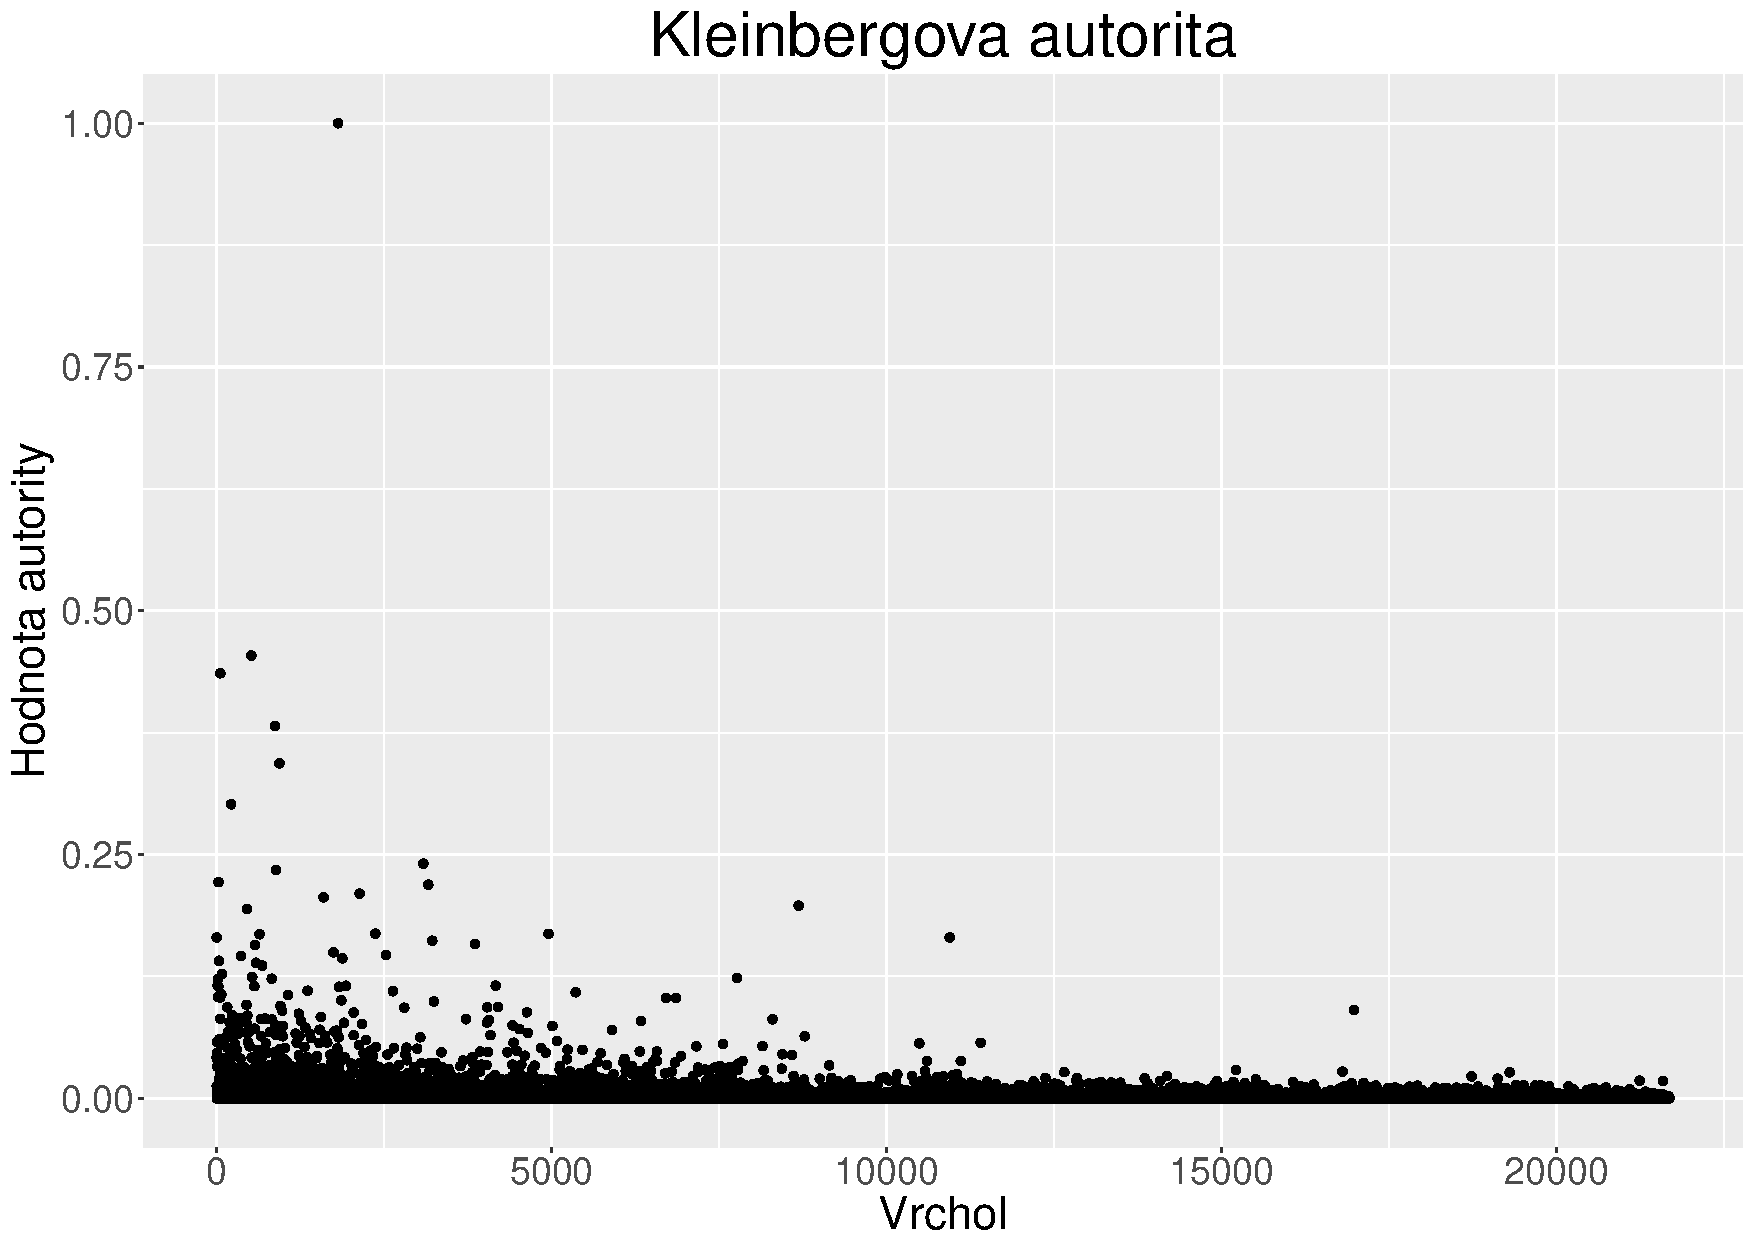
\includegraphics[scale=0.4]{images/autority.pdf}
\caption{Kleinbergova autorit centralita}
\label{img:autority}
\end{figure}

\FloatBarrier
\subsubsection{Shlukování}
V naší sítí je globální shlukovací roven 0,0501. Shlukovací koeficient jednotlivých vrcholů je už 
velmi různorodý jak můžeme vidět na Obrázku v grafu \ref{img:cluster}. Izolované vrcholy mají v tomto
grafu hodnotu 0.

\begin{figure}[h!]
\centering
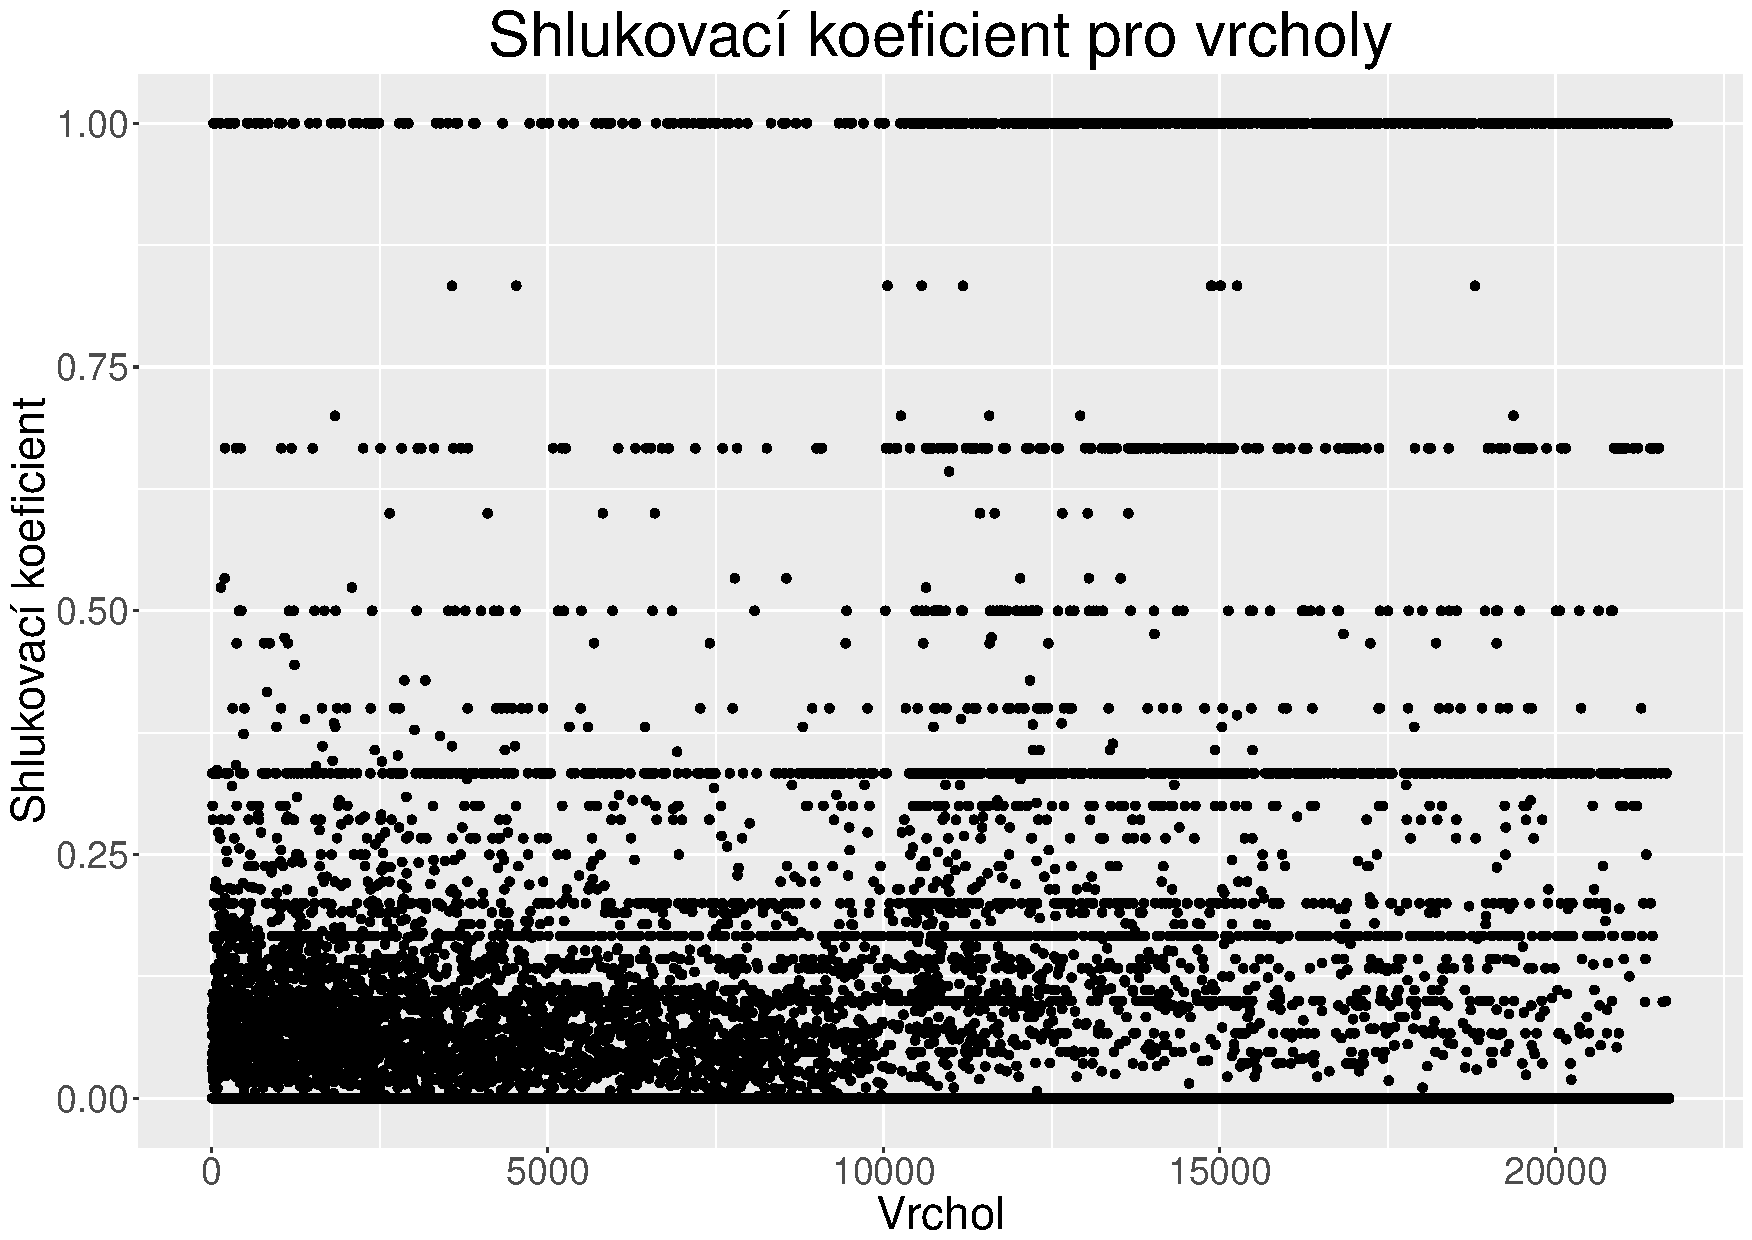
\includegraphics[scale=0.4]{images/clustering.pdf}
\caption{Shlukovací koeficient vrcholů}
\label{img:cluster}
\end{figure}

\begin{table}[h!]
\centering
\begin{tabular}{l | r | r}
		&	Hodnota	& Výskyt \\
\hline
Minimum	&	$0$			& $14 847 \times$ \\
Maximum	&	$1$			& $767 \times$	\\
Průměr	&	$0,0821$	&
\end{tabular}
\caption{Shlukovací koeficient}
\label{tab:cluster}
\end{table}

\newpage
\section{Závěr}
V námi analyzované sítí jsme objevili dvě skupiny uživatel. Pasivní uživatele a aktivní uživatele.
U aktivních je větší pravděpodobnost, že budou více odpovídat na otázky, u pasivních je to přesně
naopak.

\bibliography{citations}
\bibliographystyle{ieeetr}

\end{document}























